\documentclass{article}
\usepackage[english]{babel}
\usepackage{blindtext}
\usepackage[margin=2.5cm]{geometry}
\usepackage{graphicx}
\graphicspath{ {./images/} }

\usepackage{xcolor}
\usepackage{tabularx}
\usepackage{hyperref}


\title{Final Project Report}
\author{Fabrizio Rossi, Mina Makar, Matteo Orsini}
\date{\today}

\newcommand{\link}[2]{{\color{blue}{\href{#1}{#2}}}}

\begin{document}

\begin{titlepage}
\clearpage\maketitle
\thispagestyle{empty}
\end{titlepage}

\section{Abstract}
In this document we present our project for the Foundations of Data Science course. Since United States is one of the busiest countries in terms of road traffic with nearly 280 million vehicles, the level of traffic is one of the reasons leading to more traffic accidents. 

In order to help traffic management, we compared the performances of several models to predict the impact on the traffic of an accident. We present an Exploratory Data Analysis of one dataset offered by Kaggle which contains about 3.5 million records of accidents, and after a feature engineering phase, we compared various models implemented using the scikit-learn library showing, which model performs the best.

\section{Introduction}
The problem we faced in our project was to predict the impact of an accident on the traffic, called severity, which goes from 1, a low impact on the traffic, to 4, an high impact on the traffic. We thought that predicting this value could be useful for an automated traffic control service, in order to take decisions according to the predicted severity. So we tried to answer the question: "What is the severity of an accident which happens in a particular place and in some particular conditions?".

\section{Related work}
As related work we inspected the several notebooks available on Kaggle and on the Web which used the same dataset, or tried to accomplish the same task. In this Medium article (\link{https://ronghui-zhou.medium.com/how-you-can-avoid-car-accident-in-2020-c9626c9b6f68}{Link}), there is an in-depth analysis of the dataset state by state, and a comparison of different models deployed on our chosen dataset where the Random Forest performed the best.

Here (\link{https://www.kaggle.com/nikitagrec/usa-accidents-plotly-maps-text-classification}{Link}), instead, there is a Kaggle notebook in which the severity of an accident is predicted using just the description.
This (\link{https://www.kaggle.com/jingzongwang/usa-car-accidents-severity-prediction}{Link}) other Kaggle notebook, presents an approach which only predicts if an accident will have severity 4 or not.
In this paper (\link{https://arxiv.org/pdf/1909.09638.pdf}{Link}) a deep neural model is proposed to predict in real-time a geographical region of reasonable size, and a fine-grained time period in which an accident could occur using an augmentation of the dataset.
This Kaggle notebook (\link{https://www.kaggle.com/davidroberts13/us-traffic-analysis-folium-rfm-wordcloud}{Link}) contains a similar work to ours but it's limited just on the Fairfield county.

In the end we used two works to compare our results: this Kaggle notebook (\link{https://www.kaggle.com/gcdatkin/automobile-accident-severity-prediction}{Link}) and this Medium article (\link{https://medium.com/@vaibhavgope02/predicting-accident-severity-with-us-accidents-dataset-4aeaaae0b0af}{Link}), which both used the same dataset to carry out our same goal using different models.

\section{Dataset analysis}
We based our work on a dataset found on Kaggle (\link{https://www.kaggle.com/sobhanmoosavi/us-accidents}{Link}), which contains about 3.5 million of records about accidents happened in the US.
In the Table \ref{tab:features}, the features contained in the dataset are shown with a brief description on the second column.

\begin{table}[h!]
\begin{tabularx}{\textwidth}{|X|X|}
\hline
\textbf{Name} & \textbf{Description} \\
\hline
ID & Unique identifier of the accident record \\
\hline
Source & API that reported the accident. Can be "Bing", "MapQuest", or "MapQuest-Bing" \\
\hline
TMC & Traffic Message Channel code, which provides a description of the accident and sometimes the impact on the traffic \\
\hline
Severity & Value between 1 and 4 which describes the impact on the traffic \\
\hline
Start\_Time, End\_Time & Report the accident time. In particular, End\_Time reports the timestamp at which the effects of the accident on the traffic flow ended \\
\hline
Start\_Lat, Start\_Lng, End\_Lat, End\_Lng & Report the GPS coordinates of the start and end point of the accident \\
\hline
Distance(mi) & The length of road affected by the accident \\
\hline
Description & Natural language description of the accident \\
\hline
Number, Street, City, County, State & Indicate the place where the accident occurred \\
\hline
Side & Show the side of the road in which the accident occurred, can be "L" for left, or "R" for right \\
\hline
Timezone & Timezone of the accident \\
\hline
Airport\_Code & Indicates the closest weather station to the location of the accident \\
\hline
Weather\_Timestamp & The time-stamp of the weather observation \\
\hline
Temperature(F), Wind\_Chill(F), Humidity(\%), Pressure(in), Visibility(mi), Wind\_Direction, Wind\_Speed(mph), Precipitation(in), Weather\_Condition & Report the conditions of the weather when the accident occurred \\
\hline
Amenity, Bump, Crossing, Give\_Way, Junction, No\_Exit, Railway, Roundabout, Station, Stop, Traffic\_Calming, Traffic\_Signal, Turning\_Loop & Report the point of interest near the accident, can be true or false \\
\hline
Sunrise\_Sunset, Civil\_Twilight, Nautical\_Twilight, Astronomical\_Twilight & Report the period of the day (day or night) according to the subcategory of twilight \\
\hline
\end{tabularx}
\caption{Dataset features description}
\label{tab:features}
\end{table}

In the attached notebook, we carried out an additional \textbf{Exploratory Data Analysis (EDA)} that we will not report in this document.

%In the rest of this section, we report the results obtained from an Exploratory Data Analysis (EDA) of the dataset.
%
%\subsection*{Accidents by state}
%
%\begin{figure}[h]
%\centering
%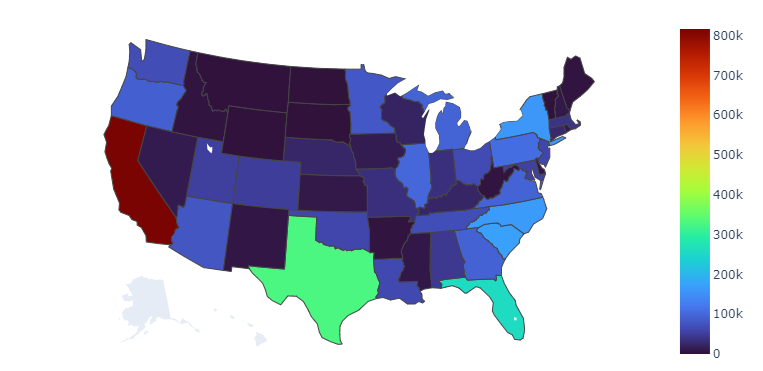
\includegraphics[width=\textwidth]{number-of-accidents-for-each-state}
%\caption{Number of accidents for each state}
%\label{img:accidents-map}
%\end{figure}
%
%We first analyzed each state of the US to check which one was the most dangerous in terms of car accidents. As we can see from the map shown in Figure \ref{img:accidents-map}, the state with the highest number of reported accidents is California, followed by Texas and Florida. This doesn't come as a surprise since they are the states with the largest population \href{https://en.wikipedia.org/wiki/List_of_states_and_territories_of_the_United_States_by_population}{(Wikipedia)}.
%
%\subsection*{Most frequent words in description}
%
%\begin{figure}[h!]
%\centering
%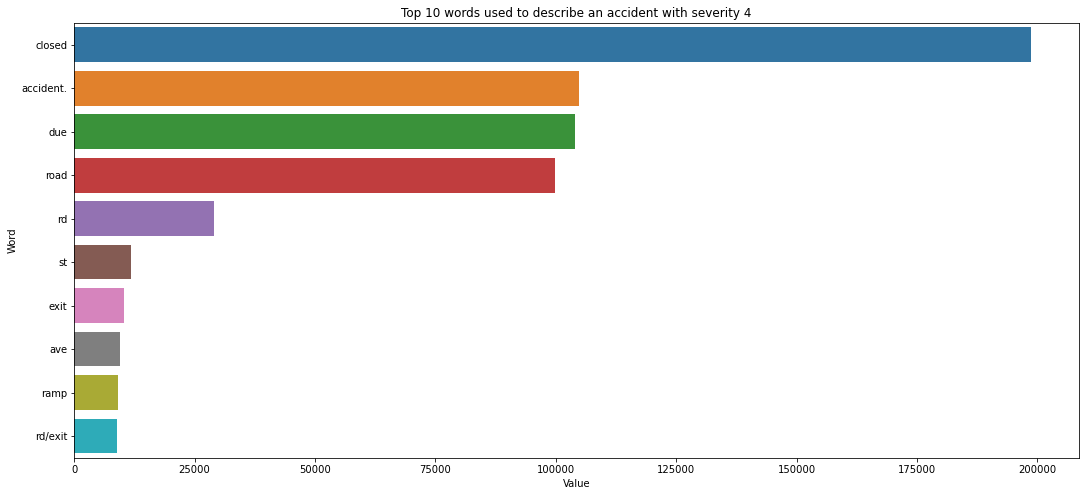
\includegraphics[width=\textwidth]{top-10-words-severity-4}
%\label{img:most-freq-words}
%\caption{Most frequent words in description of severity 4 accidents}
%\end{figure}
%
%Then, we analyzed the textual description of accidents with the maximum severity (4). From the plot shown in Figure \ref{img:most-freq-words}, we can state that the most frequent word is "closed", followed by "accident", "due" and "road".
%
%\subsection*{Most frequent road features}
%
%\begin{figure}[h!]
%\centering
%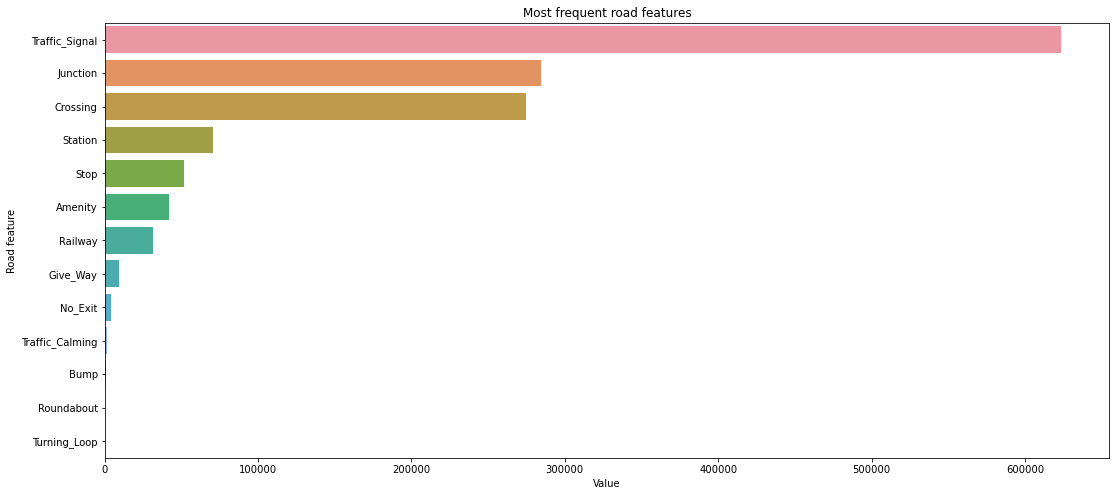
\includegraphics[width=\textwidth]{most-frequent-road-features}
%\label{img:most-freq-road-features}
%\caption{Most frequent road features}
%\end{figure}
%
%In Figure \ref{img:most-freq-road-features}, we show which road features are most frequently present in the accidents occurred. As we can see, most accidents occurred when a traffic signal was nearby, while at the second and third position, we can see that we have accidents happened near a junction or a pedestrian crossing.
%
%\subsection*{Medium distance}
%
%\begin{figure}[h!]
%\centering
%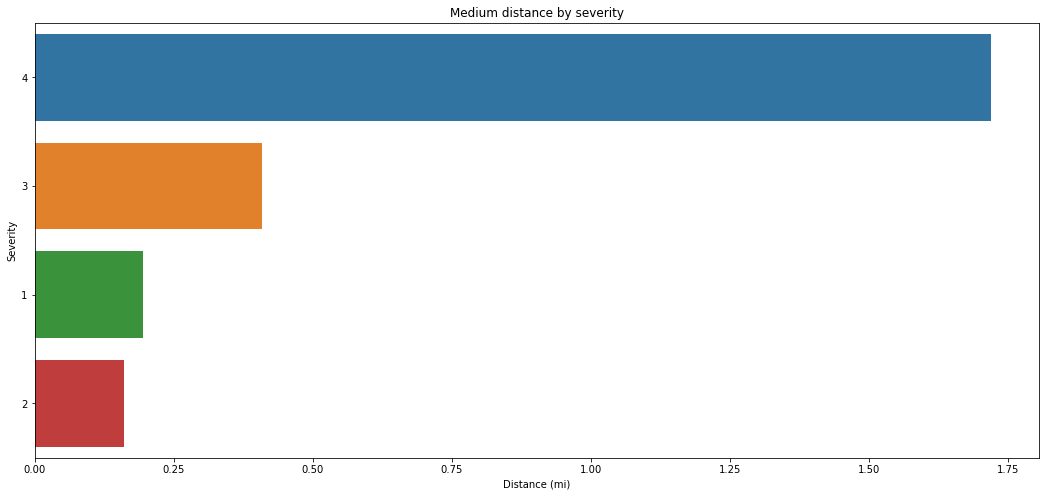
\includegraphics[width=\textwidth]{medium-distance-by-severity}
%\label{img:medium-distance}
%\caption{Medium distance for each severity}
%\end{figure}
%
%Continuing the analysis, we inspected the distance of the accidents based on their severity. The results are showed in Figure \ref{img:medium-distance}, where we can see the medium distance for each severity category. As expected, the distance is proportional to the severity of the accident, meaning that in average an accident with severity 4 is caused by a accident which affected a long portion of the road.
%
%
%
%\subsection*{Weather conditions}
%
%\begin{figure}[h!]
%\centering
%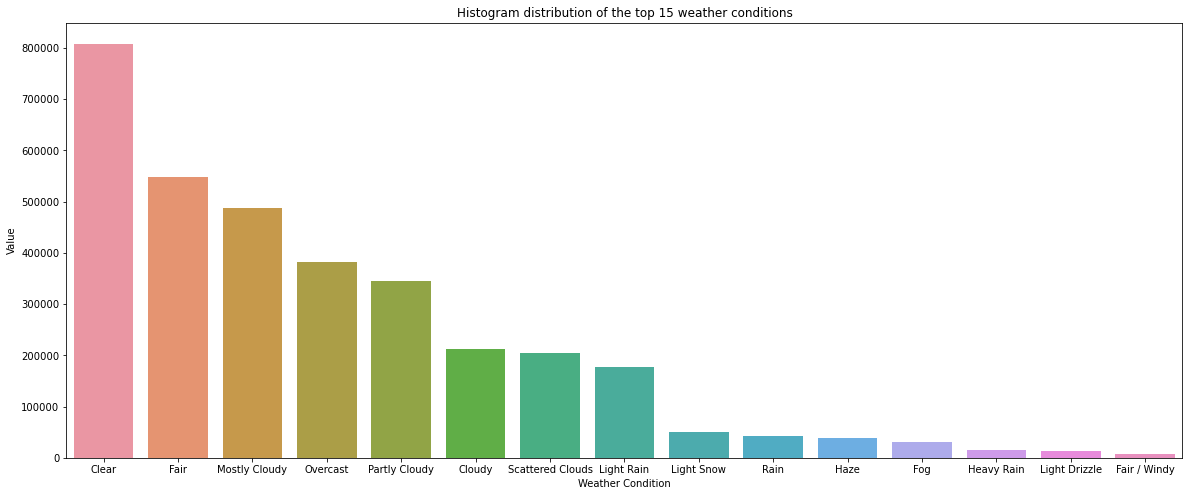
\includegraphics[width=\textwidth]{top-15-weather-conditions}
%\label{img:weather-conditions}
%\caption{Most frequent weather conditions}
%\end{figure}
%
%Then, we studied the most frequent weather conditions in which the various accidents occurred. As we can see in Figure \ref{img:weather-conditions}, in contrast to our expectations, most accidents happened with a clear, or cloudy sky.
%
%\subsection*{Accidents for each weekday}
%
%In conclusion, we analyzed the accidents distribution over the weekdays.
%From the histogram in Figure \ref{img:weekdays}, we can see that work days are the most dangerous in terms of accidents, while weekend is the safest. We were not expecting this result since during the weekend, especially teenagers, tend to not follow the rules of the streets, driving after drinking. However, the result obtained could be justified by the fact that during work days there is a greater number of cars in the streets in general, and this could be the cause of more accidents.
%
%\begin{figure}[h!]
%\centering
%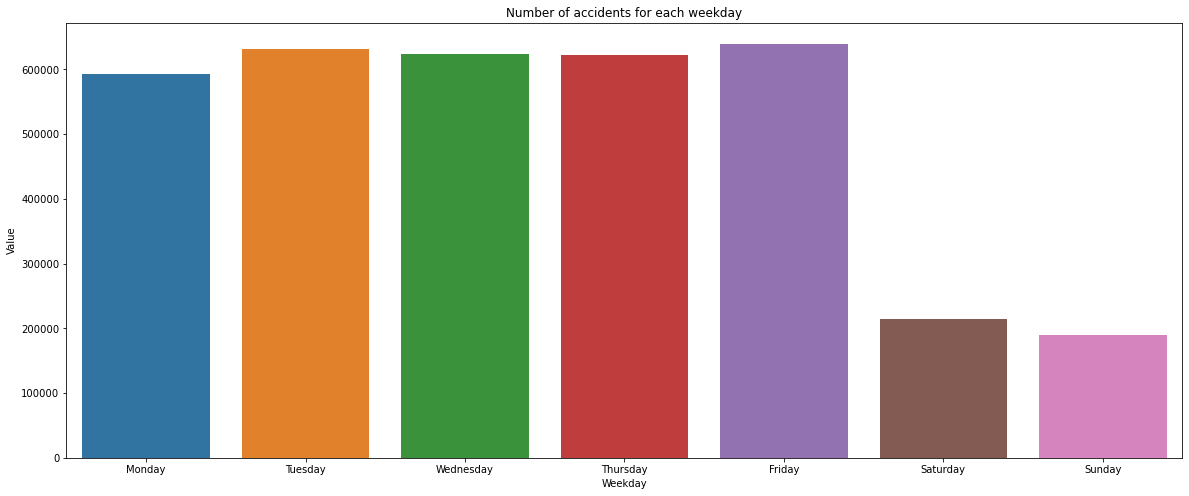
\includegraphics[width=\textwidth]{number-of-accidents-for-each-weekday}
%\label{img:weekdays}
%\caption{Number of accidents for weekday}
%\end{figure}


\section{Proposed strategy}
In this section we will describe our methodology of work to treat the features included in the dataset.
First of all, we decomposed the \textbf{Start\_Time} feature in year, month, day, weekday, hour and minutes, in order to feed them to the models.

Then, we computed the \textbf{correlation matrix} among all the feature, to inspect if we could remove some features highly correlated.

From the matrix, shown in Figure \ref{img:corr-matrix}, we can see that the start and end GPS coordinates of the accidents are highly correlated.

In fact, from the medium distance shown in the EDA, the end of the accident is usually close to the start, so we dropped the end GPS coordinates.

Moreover, the wind chill is directly proportional to the temperature, so we decided to drop the \textbf{Wind\_Chill(F)}.

From the matrix we can also note that we couldn't compute the covariance with \textbf{Turning\_Loop}, and that's because it's always False.

Upon a further analysis, we also decided to drop the following features for the reasons reported:

\begin{itemize}
\item \textbf{ID, Source}: since they don't carry any information for the severity, and we wanted to reduce the number of features;
\item \textbf{TMC}: because it could already contains information about the accident severity that should be not available for the prediction when an accident is reported. For example, TMC 106 means "stationary traffic for 10 km", but we should not have this information, since it's our goal to predict it;
\item \textbf{End\_Time}: because we cannot know in advance when the traffic flow will become regular again;
\item \textbf{Description}: most descriptions only report the name of the road of the accident, and so we decided to omit this feature for simplicity;
\item \textbf{Number, Street, County, State, Zipcode, Country}: because we just focus on the City where the accident happened;
\item \textbf{Timezone, Airport\_Code, Weather\_Timestamp}: because we think they are not useful for our task;
\item \textbf{Turning\_Loop}: since it's always False;
\item \textbf{Sunrise\_Sunset, Nautical\_Twilight, Astronomical\_Twilight}: because they are redundant.
\end{itemize}

\begin{figure}[h!]
\centering
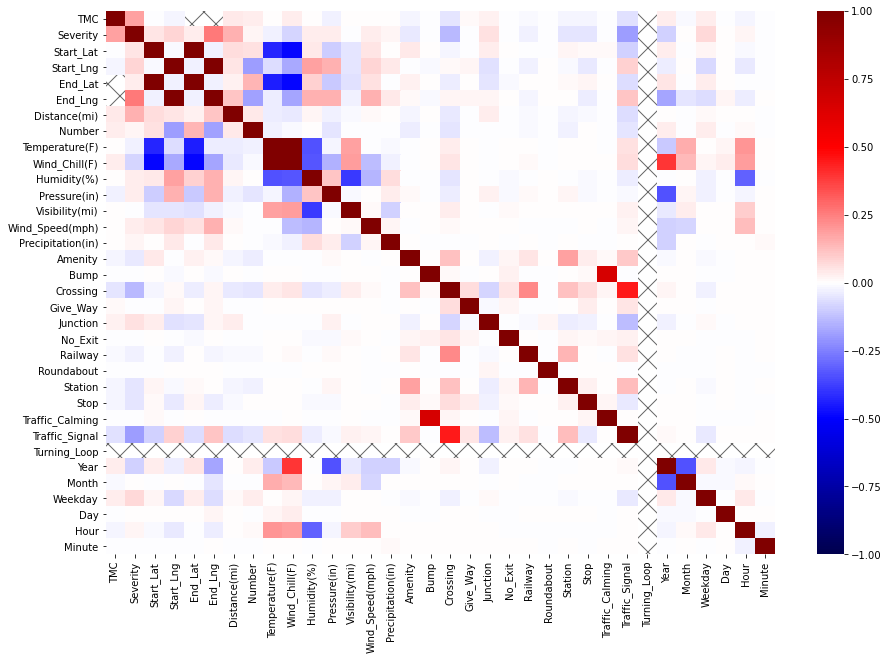
\includegraphics[width=\textwidth]{correlation-matrix}
\caption{Correlation matrix between the dataset features}
\label{img:corr-matrix}
\end{figure}

Then, we \textbf{removed duplicated} records and we inspected the dataset to check if there were some anomalous or missing values.
We \textbf{fixed some errors} in the Pressure(in) and the Visibility(mi) features, by removing records with impossible values, and we reduced the number of weather conditions and wind directions by combining similar but not equal values to reduce the number of classes for those features. 

In the end we \textbf{fixed missing values}, by filling them with the mean, for numerical features, and by dropping the entire record for categorical values, since the dataset contains lots of data.

At this point, we were almost ready to feed the dataset to the Machine Learning models, but first we needed to handle a few more aspects.

The most important of all was the number of records for each severity: as we can see from Figure \ref{img:unbalanced-dataset} the dataset was highly unbalanced.

For this reason, we used the \textbf{undersampling} technique to even the number of records to the minority class which is severity 1. After the operation, each class contained about 26.000 records.

Then, we proceeded to \textbf{scale the numerical features} using the MinMaxScaler, and to \textbf{encode the categorical ones}: boolean features were encoded simply transforming false and true to 0s and 1s; the remaining ones were encoded using the one-hot encoding except City, which was encoded using binary encoding since it would have produced too many columns (about 12.000).

\begin{figure}[h!]
\centering
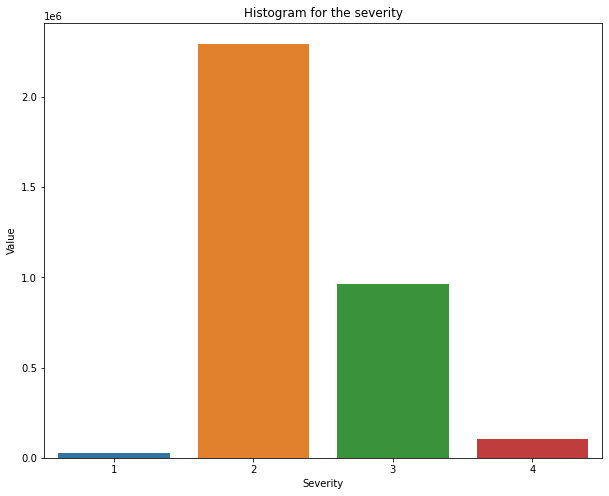
\includegraphics[width=0.6\textwidth]{unbalanced-dataset}
\caption{Number of records for each severity}
\label{img:unbalanced-dataset}
\end{figure}

\section{Experimental results}
In this section we present the results obtained with several Machine Learning models.

We \textbf{split the dataset} into three parts: 64\% of the records formed the training set, which was used to train the models, 16\% formed the validation set, used to tune the hyperparameters, and the remaining 20\%, formed the test set, used to evaluate the best model.

We tested the following models to find the best one:

\begin{itemize}
\item Logistic Regression;
\item Support Vector Machine;
\item Decision Tree;
\item Random Forest;
\item Naive Bayes;
\item Multi-Layer Perceptron.
\end{itemize}

For each model we tuned the hyper-parameters on the validation set, either by using the grid search or by checking manually some values.

For the \textbf{Logistic Regression} model, we experimented with the following solvers: Newton's solver, SAG and SAGA. We obtained the same accuracy scores , but Newton's solver took almost four times to run due to the computational power required to compute the inverse of the Hessian matrix.

Hyper-parameters tuning for the \textbf{SVM} was conditioned by the high computational cost needed by the training of the SVM. So, we used a small number of records to feed the grid search, and the best parameters found could be not the true best parameters for the entire dataset. For 5.000 records, the best parameters are: C = 1.0, kernel = polynomial with degree 2.

With respect to the \textbf{Decision Tree} model, we saw that without limiting its max depth, we would get a little bit of over-fitting since we scored 100\% accuracy on the train set, while obtaining 68\% accuracy on the validation set. Using 10 as max depth, we reduced the over-fitting obtaining an higher accuracy of 74\% on the validation set.

For the \textbf{Random Forest}, we saw that increasing the number of estimators and the max depth, we obtained better results, but increasing the risk of over-fitting. We obtained the best results using 500 estimators and 30 as maximum depth for each tree.

We saw that for \textbf{Naive Bayes} models, the best one is the Bernoulli Naive Bayes probably because most of the feature are just binary features which can assume 0s or 1s as values.

For the \textbf{MLP} we tested the architecture, the solver, the activation functions and the number of epochs. From the results we could only see that Adam solver obtains slightly better results than SGD.

The accuracy obtained by each model on the validation set is shown in the Figure \ref{img:accuracy}. Logistic Regression, SVM and Bernoulli Naive Bayes have comparable performances while the most successful models are the tree based ones: the Decision Tree and Random Forest. We can see that the latter is the best performer followed by the Multi-Layer Perceptron.

\begin{figure}[h!]
\centering
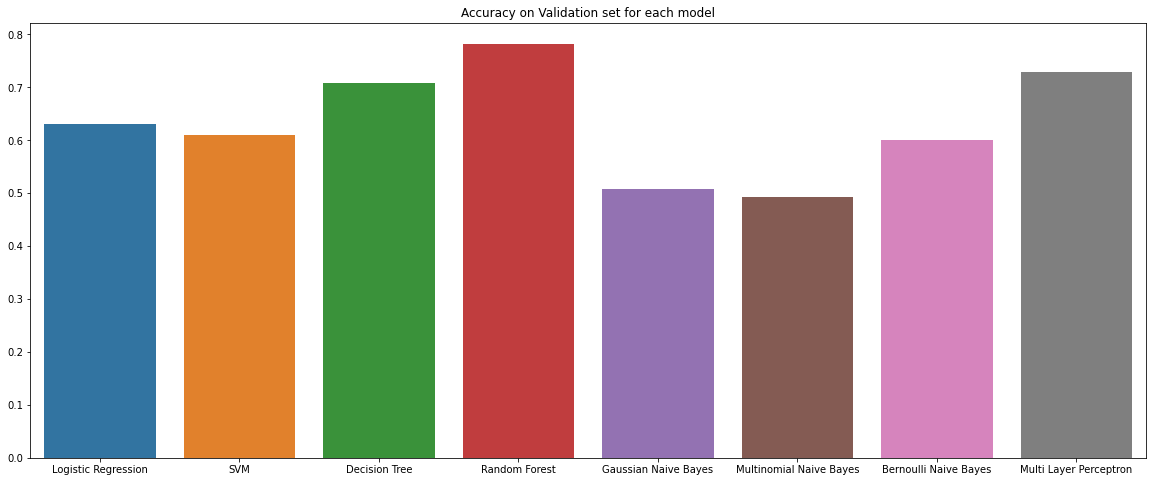
\includegraphics[width=\textwidth]{accuracy-valset}
\caption{Accuracy obtained for each model}
\label{img:accuracy}
\end{figure}

In Figure \ref{img:roc-curve} and \ref{img:pr-curve}, we can see respectively the ROC and Precision-Recall curves for each model, confirming what we said about the accuracy.

\begin{figure}[h!]
\centering
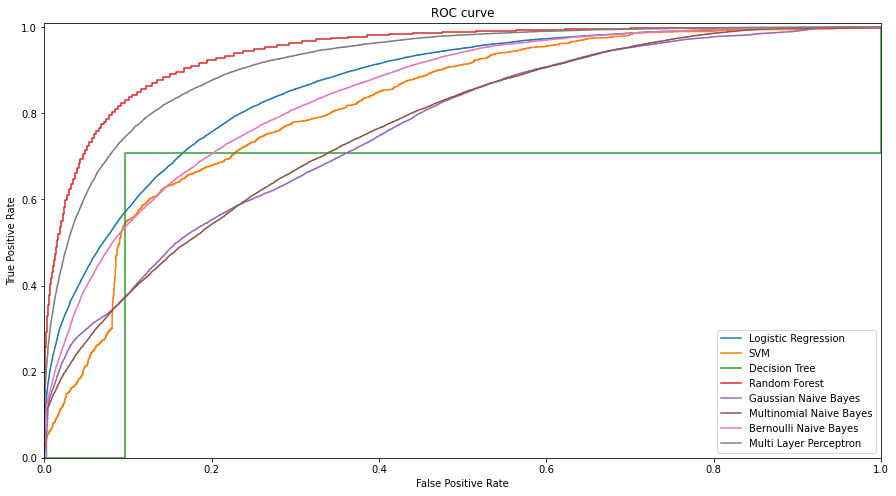
\includegraphics[width=0.8\textwidth]{roc-curve}
\caption{ROC Curves computed for each model}
\label{img:roc-curve}
\end{figure}

\begin{figure}[h!]
\centering
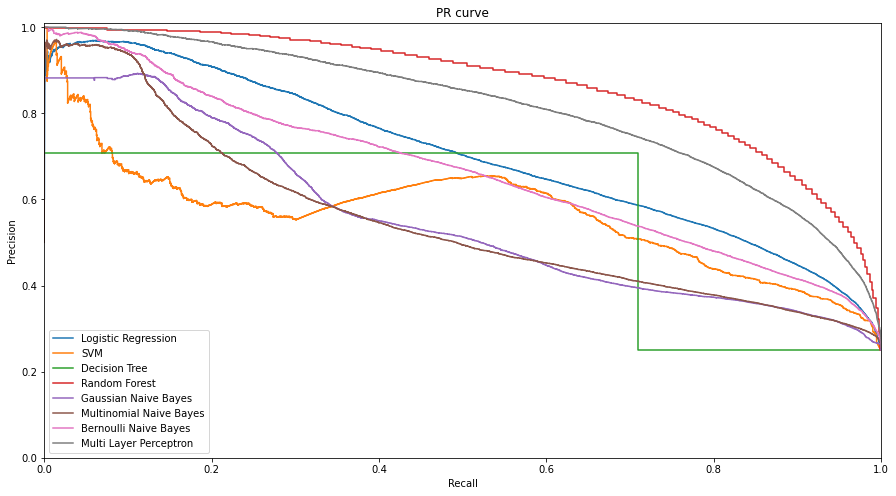
\includegraphics[width=0.8\textwidth]{pr-curve}
\caption{Precision-Recall Curves computed for each model}
\label{img:pr-curve}
\end{figure}

Since the \textbf{Random Forest} is the best model for our task, we also computed the confusion matrix, depicted in Figure \ref{img:conf-matrix}, where we can see that the most accurately classified classes are severity 1 and 4. In the Table \ref{tab:random-forest-testset}, instead, we reported the metrics collected from this model on the test set.

\begin{table}[h!]
\center
\begin{tabular}{|c|c|c|c|}
\hline
\textbf{Class} & \textbf{Precision} & \textbf{Recall} & \textbf{F1-Score} \\
\hline
1 & 0.88 & 0.95 & 0.91 \\
\hline
2 & 0.73 & 0.57 & 0.64 \\
\hline
3 & 0.69 & 0.63 & 0.66 \\
\hline
4 & 0.73 & 0.91 & 0.81 \\
\hline
\hline
\textbf{Macro-AVG} & 0.76 & 0.76 & 0.75\\
\hline
\end{tabular}
\caption{Precision, Recall, F1-Score for the Random Forest model computed on the test set}
\label{tab:random-forest-testset}
\end{table}

\begin{figure}[h!]
\centering
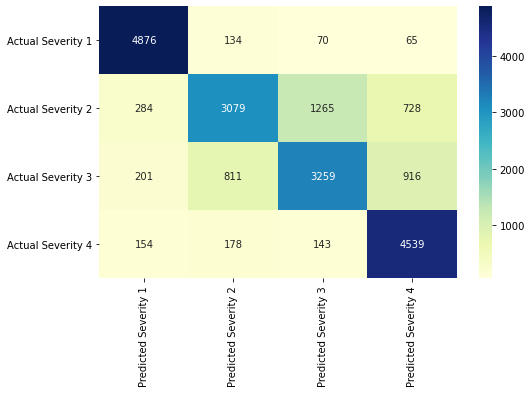
\includegraphics[width=0.5\textwidth]{best-model-testset}
\caption{Confusion matrix of Random Forest model on test set}
\label{img:conf-matrix}
\end{figure}

In the end, in the Figure \ref{img:acc-comp}, we present a comparison between our best model, the Random Forest, which obtained 76\% as the accuracy, and a few models that we found inspecting the related works that used the same dataset.
As we said in the related work section, we found a Kaggle notebook reporting the results obtained using a Neural Network and a Medium article which used several models to accomplish the same task as us.

\begin{figure}[h!]
\centering
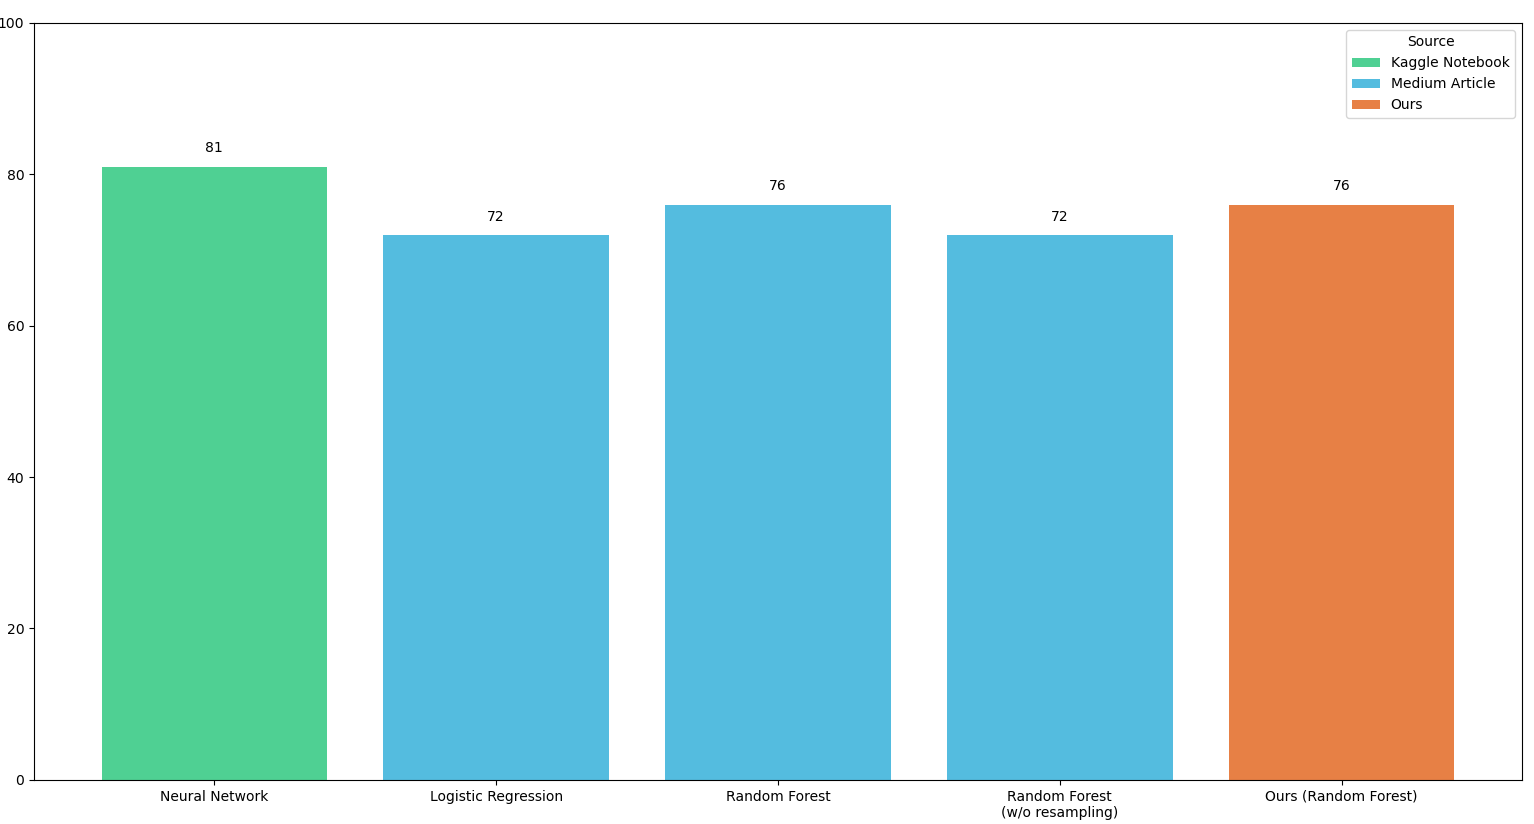
\includegraphics[width=\textwidth]{accuracy-comparison}
\caption{Accuracy comparison between different related models}
\label{img:acc-comp}
\end{figure}

\section{Conclusions}

In conclusion, we can say that accidents with severity 2 and 3 are the most difficult to predict as shown by the confusion matrix for each model. Instead, when the accident has a severity of 1 or 4, the prediction is more accurate as shown by the precision and recall of those classes.

\section{Contributions}

\subsection*{Mina Makar}
\begin{itemize}
\item Exploratory Data Analysis:
	\begin{itemize}
	\item Most frequent words in the description of an accident with severity 4
	\item Number of accidents for weekday
	\end{itemize}
\item Data preprocessing:
	\begin{itemize}
	\item Handle unbalanced data
	\item Feature scaling
	\end{itemize}
\item Model:
	\begin{itemize}
	\item Logistic Regression
	\item Decision Tree
	\end{itemize}
\end{itemize}

\subsection*{Matteo Orsini}
\begin{itemize}
\item Exploratory Data Analysis:
	\begin{itemize}
	\item Number of Accidents per State
	\item Weather condition histogram
	\end{itemize}
\item Data preprocessing:
	\begin{itemize}
	\item Feature addition
	\item Drop duplicates
	\item Feature encoding
	\end{itemize}
\item Model:
	\begin{itemize}
	\item Support Vector Machine
	\item Random Forest
	\item Multi Layer Perceptron
	\end{itemize}
\end{itemize}

\subsection*{Fabrizio Rossi}
\begin{itemize}
\item Exploratory Data Analysis:
	\begin{itemize}
	\item Most frequent road features
	\item Medium distance by severity
	\end{itemize}
\item Data preprocessing:
	\begin{itemize}
	\item Check correlation between features
	\item Handle erroneous and missing values
	\item Check feature variance
	\end{itemize}
\item Model:
	\begin{itemize}
	\item Gaussian Naive Bayes
	\item Bernoulli Naive Bayes
	\item Multinomial Naive Bayes
	\end{itemize}
\end{itemize}

\end{document}

